% Standalone source of the figure fig:lattice of the continuum-limit paper.
% Build: pdflatex fig_lattice.tex (or lualatex); the paper includes the PDF.
\documentclass[border=2pt]{standalone}
% Shared preamble of the continuum-limit paper's standalone figures.
\usepackage{amsmath,amssymb,bm}
\usepackage{tikz}
\usetikzlibrary{calc}
\newcommand{\bS}{\mathbf{S}}
\newcommand{\bG}{\mathbf{G}}
\newcommand{\bK}{\mathbf{K}}
\newcommand{\bP}{\mathbf{P}}
\newcommand{\sinc}{\operatorname{sinc}}

\begin{document}
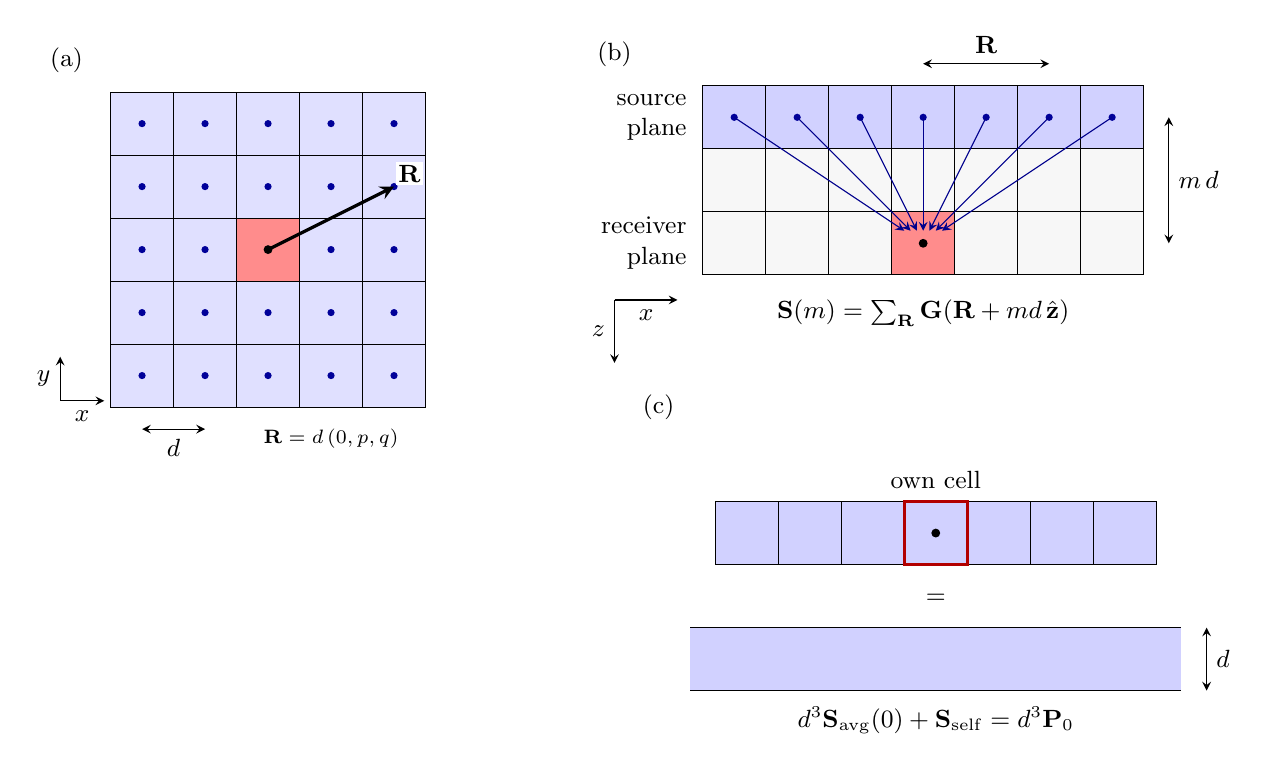
\begin{tikzpicture}[>=stealth, x=0.8cm, y=0.8cm, font=\small]
  % (a) plan view of one plane: the voxel centres form a square lattice of pitch d
  \begin{scope}[shift={(-10.4,-2.6)}]
    \foreach \p in {-2,...,2} \foreach \q in {-2,...,2} {
      \draw[fill=blue!12] (\p-0.5,\q-0.5) rectangle (\p+0.5,\q+0.5);
      \fill[blue!60!black] (\p,\q) circle (1.3pt);
    }
    \draw[fill=red!45] (-0.5,-0.5) rectangle (0.5,0.5);
    \fill (0,0) circle (1.6pt);
    \draw[->, very thick] (0,0) -- (2,1) node[above right, fill=white, inner sep=1pt] {$\mathbf R$};
    \draw[<->] (-2,-2.85) -- node[below] {$d$} (-1,-2.85);
    \node[below, align=center, font=\scriptsize] at (1.0,-2.7) {$\mathbf R=d\,(0,p,q)$};
    \draw[->] (-3.3,-2.4) -- node[below] {$x$} (-2.6,-2.4);
    \draw[->] (-3.3,-2.4) -- node[left] {$y$} (-3.3,-1.7);
    \node at (-3.2,3.0) {(a)};
  \end{scope}
  % (b) between planes: a receiver in plane m sees every voxel of the source plane
  \begin{scope}
    \foreach \c in {-3,...,3} {
      \draw[fill=blue!18] (\c-0.5, 0) rectangle (\c+0.5, -1);
      \draw[fill=gray!6]  (\c-0.5,-1) rectangle (\c+0.5, -2);
      \draw[fill=gray!6]  (\c-0.5,-2) rectangle (\c+0.5, -3);
    }
    \draw[fill=red!45] (-0.5,-2) rectangle (0.5,-3);
    \fill (0,-2.5) circle (1.6pt);
    \foreach \c in {-3,...,3} { \fill[blue!60!black] (\c,-0.5) circle (1.3pt);
      \draw[->, blue!55!black, thin] (\c,-0.5) -- ($(\c,-0.5)!0.9!(0,-2.5)$); }
    \draw[<->] (3.9,-0.5) -- node[right] {$m\,d$} (3.9,-2.5);
    \draw[<->] (0,0.35) -- node[above] {$\mathbf R$} (2,0.35);
    \node[left, align=right] at (-3.6,-0.5) {source\\plane};
    \node[left, align=right] at (-3.6,-2.5) {receiver\\plane};
    \draw[->] (-4.9,-3.4) -- node[below] {$x$} (-3.9,-3.4);
    \draw[->] (-4.9,-3.4) -- node[left] {$z$} (-4.9,-4.4);
    \node[below] at (0,-3.25) {$\bS(m)=\sum_{\mathbf R}\bG(\mathbf R+m d\,\hat{\mathbf z})$};
    \node at (-4.9,0.5) {(b)};
  \end{scope}
  % (c) within a plane: every cell, the receiver's own included, sums to a uniform plate
  \begin{scope}[shift={(0.2,-5.6)}]
    \foreach \c in {-3,...,3} \draw[fill=blue!18] (\c-0.5,-1) rectangle (\c+0.5,-2);
    \draw[very thick, red!70!black] (-0.5,-1) rectangle (0.5,-2);
    \fill (0,-1.5) circle (1.6pt);
    \node[above] at (0,-0.95) {own cell};
    \node at (0,-2.55) {$=$};
    \fill[blue!18] (-3.9,-3.0) rectangle (3.9,-4.0);
    \draw (-3.9,-3.0) -- (3.9,-3.0) (-3.9,-4.0) -- (3.9,-4.0);
    \draw[<->] (4.3,-3.0) -- node[right] {$d$} (4.3,-4.0);
    \node[below] at (0,-4.1) {$d^3\bS_{\mathrm{avg}}(0)+\bS_{\mathrm{self}}=d^3\bP_0$};
    \node at (-4.4,0.5) {(c)};
  \end{scope}
\end{tikzpicture}
\end{document}
